%%% Preamble
\documentclass[paper=a4, fontsize=11pt]{scrartcl}	% Article class of KOMA-script with 11pt font and a4 format
\usepackage[T1]{fontenc}
\usepackage{lmodern}

\usepackage[english]{babel}				% English language/hyphenation
\usepackage[protrusion=true,expansion=true]{microtype}	% Better typography
\usepackage{amsmath,amsfonts,amsthm}			% Math packages
\usepackage[pdftex]{graphicx}				% Enable pdflatex
\usepackage{url}

\usepackage[hyperref=true, sorting=none]{biblatex}
\bibliography{references}

%%% Custom sectioning (sectsty package)
\usepackage{sectsty}					% Custom sectioning (see below)
\allsectionsfont{\centering \normalfont\scshape}	% Change font of al section commands

%%% Nice tables
\usepackage{booktabs}

%%% Packages for drawings
\usepackage{tikz}
\usetikzlibrary{chains,positioning,fit,decorations.pathreplacing,shapes,calc,shadows,fadings}

%%% path to images
\graphicspath{ {images/} }


%%% some colors
\definecolor{grey}{rgb}{0.5,0.5,0.5}
\definecolor{darkgreen}{rgb}{0.078,0.667,0.016}
\definecolor{gold}{rgb}{0.85,0.65,0}
\definecolor{deepgreen}{rgb}{0.,0.5,0.}


%%% Custom headers/footers (fancyhdr package)
\usepackage{fancyhdr}
\pagestyle{fancyplain}
\fancyhead{}				% No page header
\fancyfoot[L]{}		% left
\fancyfoot[C]{}			% center
\fancyfoot[R]{\thepage}		% Pagenumbering
\renewcommand{\headrulewidth}{0pt}			% Remove header underlines
\renewcommand{\footrulewidth}{0pt}			% Remove footer underlines
\setlength{\headheight}{13.6pt}


%%% Equation and float numbering
\numberwithin{equation}{section}		% Equationnumbering: section.eq#
\numberwithin{figure}{section}			% Figurenumbering: section.fig#
\numberwithin{table}{section}           	% Tablenumbering: section.tab#

%%% List spacing
\usepackage{enumitem}
\setlist{noitemsep} % \setlist{nolistsep} for least space or \setlist{noitemsep} to leave space around whole list

%%% Maketitle metadata
\newcommand{\horrule}[1]{\rule{\linewidth}{#1}} 	% Horizontal rule

\title{
		%\vspace{-1in} 	
		\usefont{OT1}{bch}{b}{n}
%		\normalfont \normalsize \textsc{} \\ [25pt]
		\horrule{0.5pt} \\[0.4cm]
		\huge Evolving the DAQ and
                Analysis Software of the AIDA Telescope: Toward high
                rates and
                \textit{one-trigger-per-particle} Operation\\
		\horrule{2pt} \\[0.5cm]
}
\author{}
\date{\today}


%%% Begin document
\begin{document}
% Define the layers for the tikz images
\pgfdeclarelayer{background} \pgfdeclarelayer{foreground}
\pgfsetlayers{background,main,foreground}

\maketitle
\section{Introduction}
The current release branch of EUDAQ (v1.X) offers a flexible and proven
framework for data taking with multiple devices in a test
beam. However, it is based on the concept of
one-trigger-per-integration-cycle\footnote{The duration of this
  integration cycle is determined by the longest-integrating device.}
and it suffers from data-rate limitations when going to high trigger
rates. Some fundamental changes going toward a v2.0 (or AIDAQ) are
needed.

To keep the amount of work needed small (for us and others) and to allow the project to
be completed in small chunks (i.e. by different people), the changes
should generally/where possible be kept
\begin{itemize}
\item backward compatible\footnote{Backward compatible meaning no
    changes to the \emph{producer's} source code on user's side needed; if any
    changes are required, these need to be well motivated, kept minor and
    have to be clearly documented. Binary compatibility with old producers or
    data files on the other hand is not being foreseen.} to existing DUT integrations,
\item minimally invasive, and
\item modular.
\end{itemize}

\section{DAQ}
\label{sec:daq}
High trigger rates will require the ability to store large amounts of
data in short time. Therefore, potentially slow links such as Ethernet
should be avoided. Allowing each device's producer to connect to its
own (local) data collector makes it possible to spread the load onto
different machines.

Furthermore, one-trigger-per-particle operation requires to take
different device's data delivery concepts and speeds into
account. For example, devices integrating over longer periods of time
will send data blocks that cover a range of triggers. This breaks the
current concept of a synchronous event number across devices.

\subsection{New data format: \emph{packets} instead of \emph{events}}
\label{sec:event}

\begin{figure}[htbp]
  \centering
  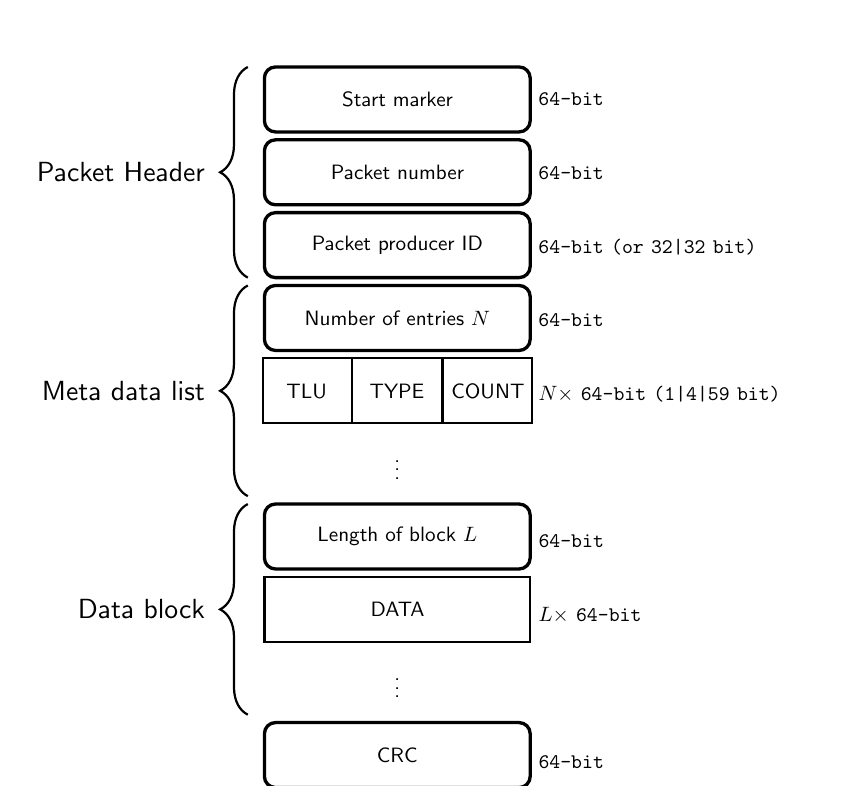
\begin{tikzpicture}[
	scale=0.75,
	start chain=1 going below, 
	start chain=2 going below,
	node distance=1mm,
	desc/.style={
		scale=0.75,
		on chain=1,
		rectangle,
		rounded corners,
		draw=black, 
		very thick,
		text centered,
		text width=4.5cm,
		minimum height=1.1cm,
                inner sep=0ex,
                outer sep=0ex
		},
	empty/.style={
		scale=0.75,
		on chain=1,
		text centered,
		text width=4.5cm,
		minimum height=1.1cm,
                inner sep=0ex,
                outer sep=0ex
		},
	listblock/.style={
		scale=0.75,
		on chain=1,
		rectangle split,
		rectangle split horizontal,
                rectangle split parts=3,
		text width=1.5cm,
		draw=black, 
		thick,
		text centered,
		minimum height=1.1cm,
                inner sep=0ex,
                outer sep=0ex
		},
	data/.style={
		scale=0.75,
		on chain=1,
		rectangle,
		text width=4.5cm,
		draw=black, 
		thick,
		text centered,
		minimum height=1.1cm,
                inner sep=0ex,
                outer sep=0ex
		},
	it/.style={
		fill=blue!10
	},
	size/.style={
		scale=0.75,
		on chain=2,
		minimum height=11mm,
		text width=5cm,
                inner sep=0ex,
                font=\ttfamily
	},
	every node/.style={font=\sffamily}
]

% PACKET HEADER
% descriptions
\node [desc] (marker) {Start marker};
\node [desc] (number) {Packet number};
\node [desc] (id) {Packet producer ID};
% sizes
\chainin (marker); % Start right of Level 5
\node [size, right= of marker] (msize) {64-bit};
\node [size] (nsize) {64-bit};
\node [size] (tsize) {64-bit (or 32|32 bit)};
\draw[decorate,decoration={brace,mirror,raise=6pt,amplitude=10pt}, thick]
    (marker.north west)--(id.south west) node [midway] (hbrace){}; 
\node[left=.5cm of hbrace] (header) {Packet Header};


% METADATA
% descriptions
\node [desc] (nentries) {Number of entries $N$};
\node [listblock] (mentry1) {TLU \nodepart{second} TYPE \nodepart{third} COUNT};
\node [empty] (lmore) {\vdots};
% sizes
\node [size] {64-bit};
\node [size] {$N\times$ 64-bit (1|4|59 bit)};
\node [size] {\phantom{\vdots}};
\draw[decorate,decoration={brace,mirror,raise=6pt,amplitude=10pt}, thick]
    (nentries.north west)--(lmore.south west) node [midway] (lbrace){}; 
\node[left=.5cm of lbrace] (list) {Meta data list};


% DATA
% descriptions
\node [desc] (length) {Length of block $L$};
\node [data] (dentry1) {DATA};
\node [empty] (dmore) {\vdots};
% sizes
\node [size] {64-bit};
\node [size] {$L\times$ 64-bit};
\node [size] {\phantom{\vdots}};
\draw[decorate,decoration={brace,mirror,raise=6pt,amplitude=10pt}, thick]
    (length.north west)--(dmore.south west) node [midway] (dbrace){}; 
\node[left=.5cm of dbrace] (data) {Data block};

% CRC
\node [desc] (crc) {CRC};
\node [size] (crcsize) {64-bit};

\end{tikzpicture}

  \caption{The new data format: packets structured into list of meta
    data (timestamps/counter values) which describes trigger and/or
    time ranges and the corresponding block of data.}
\label{fig:packetformat}
\end{figure}

Instead of sending the data in \emph{events} corresponding to single
triggers, producers send the data in \emph{packets} which can cover
arbitrary number of triggers and/or time ranges. This allows to
integrate different DAQ concepts into EUDAQ, such as untriggered or
data-driven devices.

The meta data format is designed to allow partial data merging on
request via a pull mechanism (see section~\ref{sec:integrity}).

\begin{itemize}
\item each device records and sends its data in arbitrary units ``natural'' to
  its operation (e.g. a set of frames for Mimosas)

\item the \textbf{packet header} consists of:
  \begin{itemize}
  \item a start marker
  \item the \emph{packet number} is set by each producer for
    every data block send to the data collector (starting at 1 for
    every run)
  \item the producer ID field describes the 
    detector/producer from which the data originate and which decoder
    to use; possibly to be divided into major and sub fields.
  \end{itemize}
\item the \textbf{meta data} to each packet consists of a length field and a
  list of counter entries with three fields: 
  \begin{itemize}
  \item \emph{TLU} bit to indicate whether or not this counter
    corresponds to a TLU signal,
  \item a \emph{TYPE} ID with a width of 4-bit which indicates the nature of the counter,
    e.g. trigger number, clock count (i.e. timestamp) of a TLU-event, or
    timestamp of begin/end of packet, and
  \item the 59-bit wide counter value.
  \end{itemize}
  This allows to store as meta data:
  \begin{itemize}
  \item a list of trigger numbers,
  \item a range in time during which the data was recorded, and/or
  \item a list of trigger timestamps.
  \end{itemize}
\item \textbf{Trailer}: A 64-bit field for storing a \emph{check sum} (optional)
  
\end{itemize}

Implications:
\begin{itemize}
\item as long as the old data format (one packet per trigger) is
  still supported, all existing DUT producers should work as expected
  after recompiling with the new underlying packet design.
\item the packet number does not (necessarily) match the trigger number
  and is not synchronous between devices. Specifically, the size and delivery rate
  of events is different for each device.
\item run control, data collectors and online monitors need to be adjusted so
  support the new format.
\end{itemize}

Remaining questions/issues/details yet to be decided:
\begin{itemize}
\item Can the packet format be introduced without having to adjust any
  code in the producers?
\item Can the old ``event'' be renamed ``packet'' for clarity and
  consistency without having to make significant code changes in
  existing producers?
\item What meta data types (\emph{TYPE} field) need to be supported?
  For current list of suggestions, see table~\ref{tab:typefield}.
\item What/how many detector/packet types (producer ID field in packet
  header) need to be supported and where should they be defined? For a list of suggestions,
  see~\ref{app:packettype}. Should the field be separated into two
  fields (e.g. each with 32-bit width), one ``major'' and one
  ``sub-id'' field? Should the values be fixed and centrally defined
  or should they be freely assignable by each producer?
\end{itemize}

  \begin{table}[htbp]
    \centering
    \begin{tabular}{cl}
    \toprule
    \textbf{TYPE} & \textbf{description} \\
    \midrule
    0000 &  internal trigger -- \emph{reserved for internal TLU usuage}\\
    0001 &  external trigger\\
    0010 &  shutter falling \\
    0011 &  shutter rising  \\
    0100 &  edge falling    \\
    0101 &  edge rising     \\
    0110 &  spill off       \\
    0111 &  spill on        \\
    1011 & start/end of packet data recording \\
    1111 & first/last trigger \emph{number} contained in packet \\
    \bottomrule
  \end{tabular}
  \caption{Codification of the meta data \emph{TYPE} field in the new
    packet format based on TLU signals\cite{tlu2014}. The specific
    value defines how the \emph{COUNT} field of the meta data entry is
    interpreted. An additional \emph{TLU} bit indicates whether or not the counter value
    is based on the central clock provided by the AIDA TLU.}
\label{tab:typefield}
\end{table}


\subsection{Spreading the load: multiple data collectors}
\label{sec:datacollectors}
In order to avoid slow network links and to be able to store data on
local machines, EUDAQ should support multiple data collectors,
i.e. one per (device) processor as illustrated in figure~\ref{fig:schematiclayout}.

\begin{figure}[htbp]
  \centering
  
  \begin{tikzpicture}[      
    terminal/.style={ rectangle,minimum size=6mm,rounded corners=3mm,
        very thick,draw=black!50,
        top color=white,bottom color=black!20},
      block/.style ={rectangle, draw=blue, thick, fill=blue!20,
        text width=5em, text centered, rounded corners,
        minimum height=4em},
      line/.style ={draw, thick, -latex,shorten >=2pt},
      cloud/.style ={draw=red, thick, ellipse,fill=red!20,
        minimum height=2.5em},
      minorcloud/.style ={draw=orange, thick, ellipse,fill=orange!20,
        minimum height=2.5em},     
      bluecloud/.style ={draw=blue, thick, ellipse,fill=blue!20,
        minimum height=2.5em}      
      ] 
      % TELESCOPE
      \node[] (telescope) {}; 
      \draw [line width=2pt,orange] ($(telescope.north)+(-0.2,.6)$) --++(0,0.5);
      \draw [line width=2pt,orange] ($(telescope.north)+(-0.3,.75)$) node (scint2) {} --++(0.2,0.25);
      \draw [line width=2pt,orange] ($(telescope.north)+(3.8,.6)$) --++(0,0.5);
      \draw [line width=2pt,orange] ($(telescope.north)+(3.7,.75)$) node (scint1) {} --++(0.2,0.25);
      \draw [line width=2pt,grey] ($(telescope.north)+(0,.3)$) --++(3.7,0);
      \draw [line width=2pt,grey] ($(telescope.north)+(-0.1,.05)$) --++(3.5,0);
      \foreach \i in {0,1,2,4,5,6} {
        \draw[blue,top color=blue,bottom color=blue!50] ($(telescope.north)+\i*(.55,0)$) -- ++ (0,1.25) -- ++ (0.3,0.3) -- ++ (0,-1.25) -- cycle;
        \node (plane\i) at ($(telescope.north)+(0.1,0.75)+\i*(.55,0)$) {};
        \draw[very thick, blue] ($(telescope.north)+\i*(.55,0)$) -- ++ (0,1.25) -- ++ (0.3,0.3);
        \draw[darkgreen, fill] ($(telescope.north)+(0.1,0.75)+\i*(.55,0)$) -- ++ (0,0.15) -- ++ (0.1,0.1) -- ++ (0,-0.15) -- cycle;
      }
      \node (dut) at ($(telescope.north)+3*(.55,0)$) {};
      \node (lastplane) at ($(telescope.north)+(0.1,0.75)+6*(.55,0)$) {};
      \draw[yellow!50,top color=gold,bottom color=yellow!50] (dut.base) -- ++ (0,1.25) -- ++ (0.3,0.3) -- ++ (0,-1.25) -- cycle;
      \draw[very thick, gold] (dut.base) -- ++ (0,1.25) -- ++ (0.3,0.3);

      %HARDWARE
      \node[terminal, bottom color=orange, above=2 of dut] (tlu) {\large TLU};
      \node[terminal, bottom color=gold,below=of dut] (dutdaq) {\large DUT DAQ};
      \node[terminal, bottom color=deepgreen,below=of dutdaq] (nidaq) {\large Telescope DAQ};
      \node[above=.3 of tlu] (hardwaretext) {\large Hardware};

      % EUDAQ
      \node[block, right=of lastplane] (dutproducer) {\large DUT Producer};
      \node[block, above=of dutproducer] (tluproducer) {\large TLU Producer};
      \node[block, below=of dutproducer] (niproducer) {\large Telescope Producer};
      \node[cloud, right=of tluproducer] (eurun) {\large Run Control};
      \node[bluecloud, below=of eurun] (datacollector1) {\large Data Collector 1};
      \node[bluecloud, below=of datacollector1] (datacollector2) {\large Data Collector 2};
      \node[minorcloud, below=of datacollector2] (onlinemon) {\large Online Monitor 1};
      \node[minorcloud, below=of onlinemon] (logcollector) {\large Log Collector};

      
      %CONNECTIONS
      %hardware connections
      \draw [<-,thick,orange] (tlu) -| (scint1);
      \draw [dashed, thick,orange] (tlu) -| ($(scint2)+(-.2,0)$) |- (dutdaq);
      \draw [dashed, thick,orange] (nidaq) -| ($(scint2)+(-.2,0)$);
      \draw [<->,deepgreen, thick] (nidaq) -| (lastplane) node[pos=0.85] (nidaqconnection) {};     
      \foreach \i in {0,1,2,4,5,6} {
      \draw [->,deepgreen, thick] (nidaqconnection.base) -| (plane\i);}
      \draw [<->,gold, thick] (dutdaq) -- (dut);
      %hardware-producer connections
      \draw[latex-latex,thick,deepgreen]  (nidaq)  -- (niproducer);
      \draw[latex-latex,thick,gold]    (dutdaq) -- (dutproducer);
      \draw[latex-latex,thick,orange] (tlu)    -- (tluproducer);
      %datacollector connections
      \draw[-latex,thick,blue] (niproducer)  -- (datacollector1);
      \draw[-latex,thick,blue] (dutproducer) -- (datacollector2);
      \draw[-latex,thick,blue] (tluproducer) -- (datacollector1);
      \draw[-latex,thick,dashed,blue] (datacollector1.east) -- ++ (0.35,0) |- (onlinemon);

      % harddisk
      \node (harddisk1) at ($(datacollector1.south) +(1.7,-.35)$) {
\includegraphics[width=0.75cm]{drive-harddisk}};
      \draw [-latex,thick,blue] (datacollector1.south)-- (harddisk1) node [sloped,below,pos=0.4,blue] {write};
      \node (harddisk2) at ($(datacollector2.south) +(1.7,-.35)$) {
\includegraphics[width=0.75cm]{drive-harddisk}};
      \draw [-latex,thick,blue] (datacollector2.south)-- (harddisk2) node [sloped,below,pos=0.4,blue] {write};

      %BACKGROUND
      \begin{pgfonlayer}{background}
        %hardware box
        \node [fill=black!20,rounded corners,fit=(scint1)(scint2)(hardwaretext)(nidaq)] {};
        \node [fill=black!10,rounded corners,fit=(scint1)(scint2)(tlu)(nidaq)] {};
        %computer image
          \node [right=of lastplane,opacity=0.2] (computer){
\includegraphics[width=.5\textwidth]{computer}};
          \node [below=2 of computer.north,opacity=0.2,red] (eudaqtext){\LARGE EUDAQ};
      \end{pgfonlayer}
      % HILFSLINIEN
      % \draw[help lines] (0,-3) grid (6,3);
      % \foreach \x in {0,...,6} {
      % \foreach \y in {-3,...,3} {
      % \node at (\x,\y) {\tiny \blue (\x,\y)};  };  };    
  \end{tikzpicture}

  \caption{Schematic layout of the proposed system with multiple data
    collectors each writing onto a separate disk.}
\label{fig:schematiclayout}
\end{figure}

Implications:
\begin{itemize}
\item Producers need to be associated with specific data collectors;
  possible approaches:
  \begin{itemize}
  \item run control assigns producers to data
    collectors; the appropriate data collector could be determined by the
    configuration file or by identical processor and data collector names.
  \item every producer is informed of every available data collector
    by run control and chooses one according e.g. to its name; this
    also allows for example the TLU producer to send its data to
    \emph{every} data collector. \textbf{Note:} Need to verify whether
    or not the producer-side modifications are limited to the
    \texttt{Producer::OnData()} implementation or if changes to actual
    producer's code would be necessary.
  \end{itemize}
\item online monitoring becomes more complicated as the data has to be
  collected from several sources (discussed in
  section~\ref{sec:online-monitoring}) but a single instance of the online monitor
  could run on each data collector as before.
\end{itemize}

Issues/to be decided:
\begin{itemize}
\item by what method should producers be associated with specific data collectors?
\item should the TLU producer's data be treated special in any way? It
  could be sent to a separate data collector or even to all that are available.
\item will one data collector per processor be required or do we have
  a (central) default one as fallback?
\item if one data collector has more than one producer assigned, how
  is the storage of the received events managed? We could foresee an
  index file containing a copy of the meta data and a seek position
  for the main binary file, allowing faster access to specific packets.
\end{itemize}


\subsection{Online data integrity checks and selected data packet reading}
\label{sec:integrity}
Depending on how the devices are integrated (i.e. whether they are running
synchronous or not), quite thorough consistency checks are
possible using the trigger and clock information from the TLU:

\begin{itemize}
\item correct trigger IDs with matching time stamp
\item correct trigger IDs
\item device active during all triggers (from time stamp ranges)
\item total number of triggers (difficult during run time if the trigger
  rates are constantly high, assessable with certainty only after run stop)
\end{itemize}

This task will be performed by a central \emph{run monitor} processor
while the retrieval of the packets will be performed by \emph{reader}
processors as shown in figure~\ref{fig:schematicreading}. These
collect packets (or optionally their meta-data only) by accessing the
files written by the data collectors and retrieving specific trigger
and clock ranges. The run monitor can write these packets to disk,
creating a sub-set of the available data corresponding to specific
triggers that would be suited for further processing by an online
monitor or an offline analysis. 

To be decided/implications/notes:
\begin{itemize}
\item the run monitor could start by requesting meta-data only by the
  readers; verifying consistency and finding common ranges suitable
  e.g. for determining correlations it could then proceed to request
  specific packets for each device from the readers (correlation logic
  only inside run monitor).
\item alternatively, the readers can find the packet(s) corresponding
  to a TLU trigger or TLU clock range on this information alone; this
  would allow e.g. the configuration of a specific reader with
  additional device-specific information (e.g. clock speed) but would
  probably require TLU information to be present inside each data
  collector's file.
\item the reader processor will use file-system access to the data
  (either on cache or on RAM disc); an index file containing all the
  packets' meta information and seek position for the main binary file
  could speed up the time needed to retrieve the desired packet.
\item if a device's DAQ does not include fully-qualified identifiers
  for the packet meta-data to associate it to a trigger (i.e. TLU
  trigger number and/or TLU clock-based timestamp or range), the
  information of the TLU might be needed to determine the correct
  packet(s); it could therefore be useful to have the TLU producer
  send its data to all data collectors
\item the association reader processor and data collector could be
  handled as discussed in section~\ref{sec:datacollectors} (e.g. by name)
\item the reader processors should be separate from the full system in
  such a way, that their crashing does not impact the data taking;
  furthermore, reader processors and run monitor should be able to
  reconnect to a running DAQ. This could be accomplished by having run
  control announce all available data collectors and log collectors to
  reconnecting processors that are neither device data-sources or
  device data-sinks and sending the currently active configuration
  file (in-run configure and start).
\item alternatively, the reader and run monitor constitute a separate
  software that does only minimally or not at all interact with the
  core EUDAQ system; this could provide benefits for the stability but
  might make integration and configuration more complicated.
\end{itemize}

This run-monitor triggered data retrieval mechanism can be modified to
include TLU-issued markers that are signaled to all connected DAQ
systems, allowing hardware-aided pre-selection of packets: this can be
performed in two steps. First, a hardware signal from the TLU to all
DAQs is issued on request to allow very fast devices to cache packets
(e.g. into a separate data collector) for later retrieval by the
\emph{run monitor}. This TLU signal is timestamped and included in the
next packet to mark it. Then, the \emph{reader processors} are
requested to send all packets containing such TLU marker timestamp. If
a DAQ does not include a timestamp for this signal in its packets,
either the run monitor or the \emph{reader} determines the device's
packet(s) that would correspond to the time/trigger range containing
the marker signal and retrieves it.


At first, only the latter mechanism (purely run-monitor-driven request
for specific trigger number or clock range) will be implemented.

\begin{figure}[htbp]
  \centering
  
  \begin{tikzpicture}[      
    terminal/.style={ rectangle,minimum size=6mm,rounded corners=3mm,
        very thick,draw=black!50,
        top color=white,bottom color=black!20},
      block/.style ={rectangle, draw=blue, thick, fill=blue!20,
        text width=5em, text centered, rounded corners,
        minimum height=4em},
      line/.style ={draw, thick, -latex,shorten >=2pt},
      cloud/.style ={draw=red, thick, ellipse,fill=red!20,
        minimum height=2.5em},
      minorcloud/.style ={draw=orange, thick, ellipse,fill=orange!20,
        minimum height=2.5em},     
      bluecloud/.style ={draw=blue, thick, ellipse,fill=blue!20,
        minimum height=2.5em}      
      ] 
      % TELESCOPE
      \node[] (telescope) {}; 
      \draw [line width=2pt,orange] ($(telescope.north)+(-0.2,.6)$) --++(0,0.5);
      \draw [line width=2pt,orange] ($(telescope.north)+(-0.3,.75)$) node (scint2) {} --++(0.2,0.25);
      \draw [line width=2pt,orange] ($(telescope.north)+(3.8,.6)$) --++(0,0.5);
      \draw [line width=2pt,orange] ($(telescope.north)+(3.7,.75)$) node (scint1) {} --++(0.2,0.25);
      \draw [line width=2pt,grey] ($(telescope.north)+(0,.3)$) --++(3.7,0);
      \draw [line width=2pt,grey] ($(telescope.north)+(-0.1,.05)$) --++(3.5,0);
      \foreach \i in {0,1,2,4,5,6} {
        \draw[blue,top color=blue,bottom color=blue!50] ($(telescope.north)+\i*(.55,0)$) -- ++ (0,1.25) -- ++ (0.3,0.3) -- ++ (0,-1.25) -- cycle;
        \node (plane\i) at ($(telescope.north)+(0.1,0.75)+\i*(.55,0)$) {};
        \draw[very thick, blue] ($(telescope.north)+\i*(.55,0)$) -- ++ (0,1.25) -- ++ (0.3,0.3);
        \draw[darkgreen, fill] ($(telescope.north)+(0.1,0.75)+\i*(.55,0)$) -- ++ (0,0.15) -- ++ (0.1,0.1) -- ++ (0,-0.15) -- cycle;
      }
      \node (dut) at ($(telescope.north)+3*(.55,0)$) {};
      \node (lastplane) at ($(telescope.north)+(0.1,0.75)+6*(.55,0)$) {};
      \draw[yellow!50,top color=gold,bottom color=yellow!50] (dut.base) -- ++ (0,1.25) -- ++ (0.3,0.3) -- ++ (0,-1.25) -- cycle;
      \draw[very thick, gold] (dut.base) -- ++ (0,1.25) -- ++ (0.3,0.3);

      %HARDWARE
      \node[terminal, bottom color=orange, above=2 of dut] (tlu) {\large TLU};
      \node[terminal, bottom color=gold,below=of dut] (dutdaq) {\large DUT DAQ};
      \node[terminal, bottom color=deepgreen,below=of dutdaq] (nidaq) {\large Telescope DAQ};
      \node[above=.3 of tlu] (hardwaretext) {\large Hardware};

      % EUDAQ
      \node[block, right=of lastplane] (dutproducer) {\large DUT Producer};
      \node[block, above=of dutproducer] (tluproducer) {\large TLU Producer};
      \node[block, below=of dutproducer] (niproducer) {\large Telescope Producer};
      \node[cloud, right=of tluproducer] (eurun) {\large Run Control};
      \node[bluecloud, below=of eurun] (datacollector1) {\large Data Collector 1};
      \node[bluecloud, below=of datacollector1] (datacollector2) {\large Data Collector 2};
      \node[minorcloud, below=of datacollector2] (logcollector) {\large Log Collector};
      \node[minorcloud, below=of logcollector] (runmonitor) {\large Run Monitor};
      \node[block, draw=black, fill=black!20, left=of runmonitor] (analysis) {\large Analysis};


      
      %CONNECTIONS
      %hardware connections
      \draw [<->,gold, thick] (dutdaq) -- (dut);
      \draw [dashed, thick,orange] (tlu) -| ($(scint2)+(-.2,0)$) |- (dutdaq);

      %hardware-producer connections
      \draw[-latex,thick,gold]    (dutdaq) -- (dutproducer) node
            [sloped,below,pos=0.5,gold] {\bf marked};
      \draw[latex-latex,thick,orange] (tlu)    -- (tluproducer);
      %datacollector connections
      \draw[-latex,thick,blue] (dutproducer) -- (datacollector2);
      \draw[-latex,thick,blue] (tluproducer) -- (datacollector1);
      \draw[-latex,thick,blue] (datacollector1.east) -- ++ (0.65,0) |-
      (runmonitor) node [sloped,above,pos=0.25,blue] {send selected data packets};
      \draw[-latex,thick,blue] (datacollector2.east) -- ++ (0.5,0) |- (runmonitor);
      % run monitor connections
      \draw[-latex,thick,red](runmonitor.south east) -- ++ (3.25,0) |-
      (tluproducer.north east)
      node [sloped,above,pos=0.25,red,rotate=180]{request \#1 via TLU
        signal};
      \draw[-latex,thick,red](runmonitor.south east) -- ++ (2.65,0) |-
      (datacollector1.north east)
      node [sloped,above,pos=0.34,red,rotate=180]{request \#2 via
        software call};
      \draw[-latex,thick,red](runmonitor.south east) -- ++ (2.65,0) |-
      (datacollector2.north east);

      \draw[-latex,thick,blue] (runmonitor.west) -- (analysis);


      % harddisk
      \node (harddisk1) at ($(datacollector1.south) +(1.7,-.35)$) {
\includegraphics[width=0.75cm]{drive-harddisk}};
      \draw [latex-,thick,blue] (datacollector1.south)-- (harddisk1) node [sloped,below,pos=0.4,blue] {read};
      \node (harddisk2) at ($(datacollector2.south) +(1.7,-.35)$) {
\includegraphics[width=0.75cm]{drive-harddisk}};

      %BACKGROUND
      \begin{pgfonlayer}{background}
        %hardware box
        \node [fill=black!20,rounded corners,fit=(scint1)(scint2)(hardwaretext)(nidaq)] {};
        \node [fill=black!10,rounded corners,fit=(scint1)(scint2)(tlu)(nidaq)] {};
        %computer image
          \node [right=of lastplane,opacity=0.2] (computer){
\includegraphics[width=.5\textwidth]{computer}};
          \node [below=2 of computer.north,opacity=0.2,red] (eudaqtext){\LARGE EUDAQ};
      \end{pgfonlayer}
      % HILFSLINIEN
      % \draw[help lines] (0,-3) grid (6,3);
      % \foreach \x in {0,...,6} {
      % \foreach \y in {-3,...,3} {
      % \node at (\x,\y) {\tiny \blue (\x,\y)};  };  };    
  \end{tikzpicture}

  \caption{Schematic layout of the proposed collection mechanism for
    reading selected data packets corresponding to specific trigger
    timestamp/number: (1) the run monitor requests meta-data from all
    readers; (2) the run monitor makes consistency
    checks on the meta data and requests data packets corresponding to
    a set of triggers/time stamps; (3) the full data packets are read by the
    readers either from disk or cache and sent to the run monitor,
    where they can be further processed e.g. by an offline analysis framework.}
\label{fig:schematicreading}
\end{figure}

To be decided/discussed:
\begin{itemize}
\item Should the reader and run monitor be implemented in the EUDAQ
  framwork or work as separate tools?
\item How could the algorithm for identifying correct data packets
  from meta data work in the various use cases and levels of TLU integration?
\item Specifically, how to treat DAQs running without TLU-synchronization?
\item How does the \emph{run monitor} access the information collected
  by the TLU producer?
\end{itemize}


\subsection{Online monitoring}
\label{sec:online-monitoring}
Online monitoring (i.e. correlation plots) potentially very difficult:

\begin{itemize}
\item data stream are now asynchronous between devices
\item data is stored at several locations
\item data blocks are potentially large i.e. spanning many triggers
\end{itemize}

However, online monitoring of a device class (e.g. all Mimosa planes)
is still possible with only minor adjustments to the current online
monitor.

Correlations, even of tracks fitted to aligned hits, could be studied
in immediate offline analysis.

Using the polling mechanism discussed before that flushes e.g. ranges of triggers to a
central location, the integrity checks could be extended to a
semi-online monitoring based on an offline analysis of the collected data.

Advantages of using the offline analysis framework:
\begin{itemize}
\item very modular approach
\item all work spent on integration benefits the later analysis
\item data is thoroughly and in more detail verified than (easily) possible
  with pure online monitoring
\end{itemize}

\section{Analysis}
\label{sec:analysis}
The analysis chain will be based on the EUTelescope framework. The
goal is to deliver time-tagged tracks from the telescope that can be
matched to the DUT data.

The conversion to LCIO, clustering, and transformation of timing
information to the TLU clock as global reference can be performed on
each data sample separately. But for track finding, all data belonging
to a given trigger needs to be present to allow spacial matching. The
work flow for the telescope data (Mimosa26 and timing reference plane)
could look as follows:

\begin{enumerate}
\item convert data to LCIO
\item use information from TLU to synchronize timing information to the
  TLU clock
\item verify that all triggers are present and have been seen at the
  correct time; correct if possible (optionally).
\item store hits in $x,y,z$ and $t_1, t_2$ coordinates, where the
  latter determine the time bin in which this hit occurred.
\item do spacial track matching, associate the smallest time interval
  found in a fitted hit with the track.
\item match time-tagged telescope tracks with DUT for analysis.
\end{enumerate}

Implications:
\begin{itemize}
\item after repeating this for all data streams, the resulting LCIO
  event corresponds to a specific trigger ID and will have data
  collections from all devices.
\item still, the final event might not be assigned a single but
  several triggers if they were issued quicker than the
  integration time of the fastest device.
\end{itemize}

Requirements/changes needed/to be discussed:
\begin{itemize}
\item make TLU information centrally available and store it in LCIO format
\item time stamps $t_1$ and $t_2$ in the LCIO event (what floating
  point precision is required?)
\item write TLU clock sync for Mimosa26 data with multiple triggers
  per frame
\item figure out how to efficiently handle multiple LCIO files and merge
  collections spanned across several events ($\rightarrow$ ask ILCSoft developers).
\item decide whether to output time-tagged telescope tracks or to
  handle data of telescope and DUT simultaneously when merging
\item produce monitoring/correlation histograms useful during data taking
\item provide geometry information up front (e.g. within EUDAQ)
\item optimize the analysis chain to work out-of-the-box in as many
  cases as possible (e.g. automatic iterative alignment)
\end{itemize}

\section{Acknowledgments}

  The research leading to these results has received funding from the
  European Commission under the FP7 Research Infrastructures project
  AIDA, grant agreement no. 262025. The support is gratefully
  acknowledged. 
  \emph{Disclaimer}: The information herein only reflects the views of its authors and not those of the European Commission and no warranty expressed or implied is made with regard to such information or its use.

\newpage
\appendix

\section{Packet header: \emph{Packet type} field values}
\label{app:packettype}
Values to be supported for the major field:
\begin{enumerate}
\item TLU
\item Mimosa26
\item ATLAS FEI-4
\item CMS Pixel
\item TimePix2
\item TimePix3
\item $\ldots$?
\end{enumerate}

\section{Mimosa Readout}

\subsection{Firmware}
\label{sec:firmware}
\begin{itemize}
\item replace existing firmware with ``official'' one from IPHC Strasbourg
\item request support for continuous readout
\item use global clock from TLU?
\end{itemize}

\subsection{Producer/connection to EUDAQ}
\label{sec:prod-eudaq}
\begin{itemize}
\item drop current NI producer and write Mimosa producer interfaced
  to Strasbourg DAQ software
\item potentially needs to run on Windows; communication to Strasbourg
  DAQ through TCP/IP interface?
\item Clocking out of the TLU trigger ID should only be performed once
  per frame maximum.
\item when packaging data to be sent to data collector, ``pad''
  buffered frames with one earlier and one later frame to guarantee
  that triggers received during the readout are contained in this data
  block.
\item record position of pivot pixel at time of trigger \emph{or} use
  global TLU clock and time-stamp beginning/end of frames
\end{itemize}

\printbibliography


%%% End document
\end{document}
